\documentclass[10pt,a4paper]{article}
\usepackage[spanish]{babel} % para que comandos como \today den el resultado en castellano
\usepackage{a4wide} % márgenes un poco más anchos que lo usual
\usepackage[conEntregas]{caratula}
\usepackage{enumitem}
\usepackage{graphicx}
\graphicspath{{/home/santiago/tps/metodos_numericos/Metodos_TP1/Informe}}

\begin{document}

\titulo{Trabajo Pr\'actico Número 1}
\subtitulo{Fotometria Estereo}

\fecha{\today}

\materia{M\'etodos Num\'ericos}

\integrante{Feliu, Santiago}{644/15}{santiagofeliu@hotmail.com}
\integrante{Cuba, Kennedy}{503/15}{kennedy.wrc@hotmail.com}
\integrante{Yan, Angel}{230/16}{angelyan96@gmail.com}
\integrante{Ingaramo, Pablo}{544/15}{pablo2martin@hotmail.com}
% Pongan cuantos integrantes quieran

\maketitle

\section{Introducci\'on Te\'orica}


\subsection{Fundamento ge\'ometrico'}
Dado que la superficie del modelo en mate es Lambertiana tiene la propiedad de que absorbe la luz uniformemente en cada punto, con lo cual la normal en el punto con mayor intensidad de luz de la superficie corresponde con la direcci\'on de la iluminaci\'on. Usamos para la calibraci\'on el modelo de la esfera porque al conocer su geometria y las intensidades en cualquier parte de su superficie podemos calcular las normales en todo punto.

Utilizaremos la tecnica de fotometria estereo que nos permite medir la posicion y distancia de los objetos con respecto al sensor(camara), es decir, obtener las coordenadas x,y,z basandonos unicamente en las propiedades reflectivas de la luz, para objetos no especualares y en un ambiente con iluminacion controlada.


\subsection{Fundamentos de los m\'etodos num\'ericos involucrados en el trabajo}


El foco de este trabajo pr\'actico es la resoluci\'on de sistemas de ecuaciones lineales.
En este trabajo utilizamos multiples m\'etodos num\'ericos que simplifican la tarea de encontrar la soluci\'on de estos sistemas. 
El m\'etodo mas com\'un es el de eliminaci\'on gaussiana para transormar al sistema de ecuaciones en otro equivalente(triangula el sistema) donde se pueden despejar las incognitas utilizando "backwards substitution". 
Estas tres operaciones basicas son multiplicar una fila por un escalar, sumar o restar un multiplo de una fila con otra y intercambiar filas. Siempre teniendo en cuenta que una fila no denota solo los coeficientes de las variables de una ecuacion sino tambien su termino independiente.




\subsubsection{Introducci\'on Te\'orica de algoritmos utilizados}

En el desarrollo se usan diferentes metodos para resolver sistemas lineales, algunos mejores que otros, siempre tratando de no perder presicion por errores de redondeo u otros incombenientes.
Los algoritmos que usamos son el algoritmo de eliminacion gaussiana, factorizacion LU, factorizacion de cholesky u otras variantes de ellos.
Un problema que no debe pasar desapercibido cuando trabajamos con operaciones aritmeticas en la computadora es el de perdida de digitos significativos. Esto ocurre porque la computadora trabaja con aritmetica de digitos finitos lo cual quiere decir que la representacion de los numeros en la computadora tienen una cantidad de digitos finitos para ser representados.
La mejor forma que nosotros encontramos de acotar este tipo de errores es implementado el metodo de pivoteo parcial en nuestro algoritmo de eliminacion gaussiana.

\subsubsection{Eliminacion Gaussiana}
El metodo de eliminacion gaussiana tiene complejidad temporal O($n^{3}$) y cuando tenemos que resolver multiples sistema de ecuaciones lineales esta complejida no es tan buena.
En la division de los pivotes, se selecciona el mas grande de entre las filas mirando en esa columna, asi al dividir por el numero mas grande el error del numero al que estoy dividiendo, no se ve tan reflejado en las cuentas ya que estoy achicando el error o no lo estoy agrandando demasiado.


\subsubsection{factorizacion LU}
Encontrar la factorizacion LU de una matriz tiene costo O($n^{3}$), la resolucion del sistema A$x$ = LU$x$ = b tiene costo O($n^{2}$), lo cual hace que en las situaciones donde hay que resolver muchas veces el sistema Ax = b para diferentes b sea mucho mas eficiente que utilizar el algoritmo de eliminacion de gauss. 
Tomamos la decision de usar la factorizacion PLU, ya que nos permite pivotear y es muy similar. 
La existencia de la factorizacion LU no esta garantizada para cualquier matriz. Las condiciones necesarias y suficientes para que exista la factorizacion LU son que no aparezca un zero como pivote a lo largo de la factorizacion LU o que todas las submatrices principales sean inversibles. Aunque la factorizacion LU no siempre existe, la factorizacion PLU si.

\subsubsection{Factorizacion Cholesky}
Esta factorizacion se usa al obtener la matriz de pixeles para buscar las profundidades, y reescribir las ecuaciones para que la nueva matriz sea una matriz definida positiva, asegurando que existe la factorizacion cholesky para la matriz con la cual podemos trabajar ya que la solucion original al sistema no cambia.

\subsubsection{Matrices Banda}
En la construccion de la matrix de pixeles(para armar el espacio normal de ecuaciones), se puede armar la matriz de tal forma que quede una matriz banda, la cual hace que la matriz tenga muchos ceros y poder optimizar algunos algoritmos en funcion de eso.


\subsubsection{Matrices Esparzas}
Para la reconstruccion 3D, como las matrices con las que trabajamos son banda y esparzas podemos utilizar una estructura en la cual la matriz considere a los elementos que no son cero y asi disminuir la complejidad tanto temporal y espacial de los algoritmos 

\subsubsection{Definiciones}
Una matriz es simetrica y definida positiva <=> tiene factorizacion cholesky



\section{Desarrollo}

Durante el desarrollo se fue observando que al trabajar con aritmetica finita se presenta la posibilidad de errores de redondeo en varias oportunidades por este motivo se decidio utilizar double's para la una mejor representacion de los números. Con lo cual se decidio utilizar una cota para este error (llamada epsilon) la cual es un numero pequeño que se utiliza para la comparación con el cero. En otros de los lugares donde tuvimos que considerar este error fue al momento de triangular las matrices en donde para cada columna se buscaba en que fila se encontraba el mayor valor, asi al restarle a las siguientes filas un multiplo del mayor valor se minimiza el error de redondeo. \\


El programa desarrollado se puede dividir en tres partes: La obtención de las direcciones de luz, la obtención del campo normal y la reconstruccion del modelo 3D.
La primera parte consiste en conseguir las direcciones de fuentes de luz y elegir de estas las que nos permitan hacer una reconstruccion optima de los modelos.
En la segunda parte utilizando las direcciones obtenidas durante la calibracion y se estiman las dirreciones normales de la superficie del modelo elegido.
Y por último se obtienen las profundidades con la utilización del campo normal obtenido en el paso anterior.

\section{Obtención de las direcciones de la luz}

\subsection{Calibración}

En el desarrollo de este trabajo práctico lo primero que hicimos fue la calibracion del sistema. Esto consistio
en encontrar las direcciones de la luz en cada una de las 12 imágenes de la esfera. Para lo cual utilizaríamos la ecuación de la esfera $r^{2}$=$(x-x_{0})^{2}$ + $(y-y_{0})^{2}$+ $(z-z_{0})^{2}$, donde los datos que podremos obtener de las imágenes serán las coordenadas ($x_{0}$,$y_{0}$) del centro de la esfera, el radio r y las coordenadas del pixel que consideramos mas brillante (x, y). Si C es el centro de la esfera y P el punto donde se encuentra el pixel mas brillante, entonces el vector que representa la dirección de la iluminación 
es C-P = ($x_{0}$ - x, $y_{0}$ - y, $z_{0}$ - ($ \sqrt{r^{2} - (x-x_{0})^{2} - (y-y_{0})^{2} + z_{0}}$)) = ($x_{0}$ - x, $y_{0}$ - y, $\sqrt{r^{2} - (x-x_{0})^{2} - (y-y_{0})^{2}}$). \\

Lo mas sencillo de la obtención de los datos será encontrar coordenadas del centro y el radio de la esfera. Para ello utilizamos la máscara donde al recorrer la imágen se logra conseguir facilmente los extremos de la esfera, con los cuales se obtiene la diferencia entre ellos y se obtiene el centro y el radio. \\

Luego, para encontrar el punto mas brillante, debiamos considerar que la visión humana tiende a diferenciar más escalas de verde lo cual implica que al hacer un promedio ponderado para el color verde se obtengan mejores resultados. Por lo tanto este promedio será la forma en la que calcularemos la luminosidad del pixel.\\

Ya teniendo en cuenta como obtener la luminosidad pasamos a la forma de encontrar el pixel mas brillante, nuestra primer idea fue analizar uno por uno todos los pixeles de cada imagen hasta encontrar el pixel con la máxima intensidad en el rango de 1 a 255.
Esto implico que al seleccionar el pixel con mayor intensidad encontramos que era posible que haya varios pixeles con la misma intensidad, lo cual solucionamos eligiendo uno al azar.
Esta solución nos implico más problemas, los cuales al analizarlos nos dimos cuenta de varias cosas, entre ellas:
\begin{itemize}
	\item  No es lógico elegir un punto al azar, ya que este representaria la dirección de la luz la cual es única.
	\item La esfera tiene irregularidades sobre su superficie, lo que genera una clase de ruido.
	\item El brillo forma una clase de aureola sobre la superficie.
\end{itemize}
A partir de estas observaciones concluimos que no alncanzaría con obtener el pixel mas brillante. Por lo tanto se decidio que utilizaríamos un promedio del brillo de los pixeles vecinos, así de esta manera poder agrandar el espectro de cada pixel.\\

Finalmente al haber consegido los puntos mas brillantes de las imágenes lograriamos obtener la incognita z de la que hablamos en un principio.


\subsection{Elección de las direcciones de la fuente de luz}

Nuestro criterio para la elección de las direcciones de luz se basa en elegir aquella combinación que tenga el menor número de condición. Por lo que aprendimos en clase una matriz mal condicionada es propensa a tener graves errores y no darnos soluciones del sistema en las cuales podemos confiar.\\
Al mismo tiempo, pensandolo de manera geométrica observamos que el condicionamiento de una matriz va a mejorar a medida que las ecuaciones lineales de la matriz esten lo mas lejano posible de ser paralelas, lo cual tiene sentido ya que tener iluminación dispersa ayuda a ver un objeto mejor en el mundo real. Nosotros suponemos que el error que vamos a obtener al calcular las normales va a estar directamente relacionado al condicionamiento de la matriz que utilizamos. Dicho de otra manera, el mejor gráfico de las normales va a estar dado por la matriz mejor condicionada.\\

Ya sabiendo cual seria el aspecto de nuestra matriz ideal nos faltaría encontrar la mas apta. Para esto  programamos un algoritmo que calcula todas las posibles permutaciones de tres vectores, teniendo 12 vectores para elegir, junto con el numero de condición asociado a cada una de estas matrices. Hay que tener en cuenta que al calcular las posibles permutaciones de las direcciones consideramos a una elección de tres vectores como un conjunto, ya que el número de condicion no cambia si permutamos las columnas o filas de una matriz.


\section{Construcción del campo normal}	


\indent Con las tres direcciones de iluminación ya elegidas el siguiente paso del desarrollo es el cálculo de las normales en cada pixel. Esta es la etapa del trabajo práctico en la cual implementamos y utilizamos los algoritmos de eliminación de gauss y la factorización LU.\par

\subsection{Eliminación Gaussiana}

\indent Nuestro algoritmo de eliminación gaussiana, hace n iteraciones donde n es la cantidad de filas de la matriz a triangular. En la i-esima iteración toma el elemento $a_{ii}$ como pivote. Si el pivote en cualquiera de las iteraciones es cero entonces no existe factorización LU pura, aunque si existe factorizacion PLU. Si el pivote no es cero el algoritmo hace otras k iteraciones donde k es la cantidad de filas que tiene por debajo. El algoritmo procede a calcular el múltiplo exacto por el cual tiene que multiplicar al pivote para poder eliminar al elemento, que este en la misma columna que el, y en la fila debajo de si. Esto lo repite k veces, una ves para cada fila que se encuentra por debajo del pivote actual. Una vez terminadas las k iteraciones para el i-esimo pivote, el algoritmo pasa al siguiente pivote. Resulta evidente que los pivotes va a ser todos los elementos de la diagonal. \par

\subsection{Factorización LU}

\indent Obtener la factorizacion LU no es mas que guardar los múltiplos que utilizamos para diagonalizar una matriz en el algoritmo de eliminación gaussiana. Es importante notar que nosotros implementamos un algoritmo de factorizacion PLU donde la factorizacion LU es el caso especifico donde la matriz P es la matriz identidad. Por lo cual, la complejidad temporal de obtener la factorizacion LU  es igual a la complejidad del algoritmo de eliminacion de gauss, la cual es O($(n)^{3}$).\par

\subsection{Diferencia entre ambos algoritmos}

\indent Aunque sus complejidades son iguales, la diferencia se encuentra al momento de resolver varios sistemas. La eliminación gaussiana va a tener la misma complejidad cada vez que la utilizamos. En contraste, la factorización LU solo se obtiene una vez y luego solo se debe resolver dos sistemas triangulares, esto lleva a que su complejidad es O($(n)^{2}$). Como dice el enunciado del TP, los valores $s_{x}$, $s_{y}$, $s_{z}$, de la ecuación 5 no cambian pixel a pixel sino que solamente se modifica el valor de la intensidad en (x,y) para la imagen correspondiente $I_{i}$, y por lo tanto poseen la misma matriz pero con distinto término independiente. Por lo cual, si se encuentra una convinación de $s_{1}$, $s_{2}$ y $s_{3}$ que posea factorización LU se podria bajar sustancialmente la complejidad de obtener las normales de una imagen, ya que estas poseen una gran cantidad de pixeles.\par


\section{Obteniención de las profundidas}	

Finalmente el último paso es resolver las ecuaciones 11 y 12, las cuales nos permiten construir un sistema de ecuaciones sobredeterminado para todo el espacio de píxeles.\par
Las ecuaciones 11 y 12 asociadas a un pixel (x,y) se puede reescribir de la siguiente manera:\par
$\begin{cases}
n_{z} z_{x+1,y} - n_{z} z_{x,y}= n_{x} \text{(11*)}\\
n_{z} z_{x,y+1} - n_{z} z_{x,y}= n_{y} \text{(12*)}
\end{cases}$
\break
\indent Utilizando las ecuaciones 11* y 12* de todos los pixeles de una imagen podemos armar un sistema sobredeterminado de la forma $Mz=v$, donde $M \in {\rm I\!R}^{2NxN}$. \par
\indent El vector $z \in {\rm I\!R}^{N}$ es un vector columna que tiene las profundidades que estamos estimando por lo cual va a tener en sus filas a las variables $z_{x,y}$ de todo pixel $(x,y)$. El vector $v \in {\rm I\!R}^{2N}$ es un vector columna que esta formado por los términos independientes de las ecuaciones 11* y 12*, por lo cual tiene en sus filas a los terminos $n_{x}$ y $n_{y}$ asociados a cada pixel de la imagen. Las filas de $M$ van a estar formadas por los coeficientes de las ecuaciones (11*) y (12*). Por lo cual cualquiera fila de $M$ que este asociado a algun pixel (x,y), va a tener todos ceros excepto en las columnas que coincidan con las variables $z_{x+1,y}$ y $z_{x,y}$ o las variables  $z_{x,y+1}$ y $z_{x,y}$, donde envez de ceros tiene los coeficientes $n_{z}$ y $-n_{z}$.\par 
\indent El sistema de ecuaciones $Mz=v$ lo transformaremos para obtener las ecuaciones normales que resuelven el problema de cuadrados mínimos $M^{t}Mz=M^{t}v$, donde la solución $z$ es el vector con las profundidades que buscamos. Al aplicar esta tranformación nos queda que la matriz $A= M^{t}M$ es simétrica definida positiva lo cual nos permite usar el método de factorización de cholesky ya que sabemos que una matriz es simetrica definida positiva si y solo si tiene factorizacion cholesky.\par

%\subsection{Armando la matriz M}

%La forma (naiv), es ver la grilla de píxeles en forma de F1++F2++...++Fn concatenacion de los pixeles (donde F1 contiene a todos los píxeles correspondiente a todas las columnas de la fila 1 de la grilla, %analogamente Fn). Con los cual, si separamos las ecuaciones y formamos 2 matrices una para las ecuaciones correspondientes al eje X y otra matriz correspondiente al eje Y. Tenemos una Matriz Banda 1x2 %Para el eje X y 1x(cantidad De Columnas de las grilla +1) para el eje Y. Combinandolos de manera adecuada, se obtiene la matriz banda(anhelada).(X1/Y1/.../Xn/Yn)

%MxMt es simetrica, es valido para toda matriz.

%\subsection{Descripcion de la matriz M }

%La matriz M tiene dimension 2NxN y es banda PxQ, por lo tanto Mt es de dimension Nx2N y es banda QxP, luego siendo A = MxMt tiene dimension NxN y es banda Qx(Q+1).
%Ya que como esta armada la matriz M, se forma una escalera donde al moverse por las columnas,mirando desde la q+1 columna, la  primer coordenada tiene el primer elemento igual a cero y todas los demas no necesariamente distinto de cero.Al mirar la siguiente columna la cantidad de elementos que no son cero incrementan en dos y asi mientras se observa la siguiente columna.
%Luego al mirar las filas, se logra encontrar un patrón en el cual se agrega un cero a las primeras coordenadas de la fila cuando se dan pasos de a dos filas. Lo cual forma un patron interesante al ser multiplicado por su transpuesta, esto relaciona la cantidad de píxeles con el ancho de banda de la matriz el cual queda dependiendo de la cantidad de píxeles y del ancho de la imágen.


%\subsection{Mirando ceros de la parte superior} 
%Para la matriz A resultante al juntar lo visto, y siguiendo la misma idea con la matriz traspuesta, se observan los mismos patrones.Por lo tanto al hacer la multiplicación, se puede observar un patrón que siguen cada una de las filas de la matriz resultante , en particular la fila i (i $\leq$ Q) tiene sus coordenadas igual a cero desde la posicion Q+i+1, eso forma una diagonal de elementos no necesariamente igual a cero a partir de la fila 1 columna q.

%\subsection{Mirando los ceros de la parte inferior} 
%Para la fila i (i $>$ Q), tiene el primer cero a partir de la fila q+1 en la coordenada 1  y va incrementando un cero a las primeras coordenada del vector fila cada ves que avanza, con lo cual eso forma una diagonal de elementos no necesariamente igual a cero a partir de la fila q columna 1.

%\subsection{Forma de la matriz resultante}
%Para obtener la matriz A que da la multiplicación de la matriz MxMt, dado que son matrices banda y que M es banda PxQ donde p=cantidad de elementos(pixeles)-1 y Q = cantidad de columnas de la imagen. Si la imagen es una tira de píxeles entonces P = Q, sino P $>$ Q.
%La matriz resultante tiene dimension NxN y es banda Qx(Q+1). 

\subsection{Justificación de utilización de la factorización de cholesky para la matriz A}

Para poder justificar cholesky, nos alcanza con demostrar que las columnas de la matriz $M$ son LI, lo cual vamos a demostrar por el absurdo.\par
\indent Supongo que $M$ tiene columnas LI $\rightarrow$ $A$ no es S.D.P. \par 
\indent Como sabemos que $M$ tiene columnas LI $\rightarrow$ $(\nexists x ) Mx = 0 \land x \neq 0 $. Por otro lado sabemos que $A$ no es SDP, luego $x^{t}Ax$ $\leq 0 \forall x \neq 0 \in {\rm I\!R}^{n}$.\par Como $A = M^{t}M \rightarrow x^{t}Ax = x^{t}M^{t}Mx = (Mx)^{t}(Mx) = ||Mx||_{2}^{2}$ ademas sabemos que $x^{t}Ax \leq 0$, entonces nos queda que $||Mx||_{2}^{2} \leq 0$. Pero por definición de norma sabemos que toda norma es mayor o igual a cero, entonces $||Mx||_{2}^{2}$ = 0, lo cual es absurdo ya que dijimos que no existe un $x \neq$ 0 tal que $Mx = 0$. Por último, utilizando la Propiedad*, tenemos que la matriz A tiene factorización cholesky única.

\subsubsection{Demostración que las columnas de la Matriz M son L.I}
\indent La matriz M se construye a partir del sistema de ecuaciones que resulta de considerar las ecuaciones 7 y 8 tomando a $z_{x,y}$ como la incognita que representa la profundiad del pixel (x,y). No se consideran los pixeles cuyo $n_{z}$=0 ya que esto seria un punto sin profundidad (z=0). \par
\indent Luego cada pixel tendria las siguientes ecuaciones:\par
$\begin{cases}
n_{z} z_{x+1,y} - n_{z} z_{x,y}=0\\
n_{z} z_{x,y+1} - n_{z} z_{x,y}=0
\end{cases}$
\break
\indent Entonces la matriz $M$ tendria en las dos filas correspondientes al pixel (x,y) a todos los valores en cero salvo las columnas correspondientes a los pixeles (x,y) y (x+1,y) o (x,y+1). \par
\indent Para ver la independencia lineal de las columnas de $M$ vamos a analizar para que soluciones $z \in {\rm I\!R}^{n}$ vale que $Mz=0$. Vamos a ver para cada pixel que valores de $z_{x,y} , z_{x+1,y}$  y $z_{x,y+1}$ dan que: \par
$\begin{cases}
n_{z} z_{x+1,y} - n_{z} z_{x,y}=0\\
n_{z} z_{x,y+1} - n_{z} z_{x,y}=0
\end{cases}$
\break
Equivalentemente:\par
$\begin{cases}
n_{z} z_{x+1,y} = n_{z} z_{x,y}\\
n_{z} z_{x,y+1} = n_{z} z_{x,y}
\end{cases}$
\break
\indent Lo cual sucede si y solo si $z_{x+1,y} = z_{x,y}$ y $z_{x,y+1} = z_{x,y}$. \par
Reemplazando (x,y) por (x+1,y) tenemos que $z_{x+2,y} = z_{x+1,y}$ y $z_{x+1,y+1} = z_{x+1,y}$ lo cual implica que $z_{x,y}=z_{x+1,y} =z_{x,y+1}= z_{x+2,y} = z_{x+1,y+1}$.\par
Esta idea se puede aplicar para cualquier par (x,y) luego tenemos que $z_{x,y} = z_{x',y'}$ para cualquier par de pixeles (x,y) y (x',y').\par
\indent Entonces  Mz=0 si las profundidades de todos los pixeles son iguales. Pero esto sucede si la imagen es "plana". En este caso no tiene sentido realizar una rescontrucción 3D, ya que no hay nada para reconstruir. Por lo cual este caso lo podemos descartar.\par
\indent Luego  $(\nexists x ) Mx = 0 \land x \neq 0 $ $\rightarrow$ las columnas de M son L.I.


%Para poder justificar cholesky, nos alcanza con demostrar que las columnas de la matriz M son Li ya que por la definición de matriz definida positiva, vale que para $w^{t}Aw$ $>$ 0 $\forall$ w $\in$ ${\rm I\!R}^{nxn}$, la demostración es por el contrarresiproco con lo cual suponemos lo contrario existe un $(\exists w ) Aw = 0 \land w \neq 0 $ , como A = $ M^{t}M \rightarrow w^{t}M^{t}=(Mw)^{t}(Mw)$ =$||Mw||^{2}$ y como esto es la norma del vector, la norma de ese vector es 0, como demostramos que las columas eran Li, con lo cual llegamos a un absurdo que provino de suponer que existe tal w, por lo tanto la matriz A es definida positiva. Y usando la Propiedad*, tenemos que la matriz A tine factorizacion cholesky unica.

Propiedad*: Una matriz es simetrica definida positiva $\leftrightarrow$ tiene factorizacion cholesky unica.





\section{Experimentaci\'on y Resultados}



\section{Vecindades}

Para poder observar cuantos pixeles vecinos debíamos tomar en cuenta para encontrar la dirección de la luz procedimos a hacer un breve experimento donde pintabamos de distintos colores los pixeles que consideraba mas brillante dependiendo la cantidad de vecindades. En este caso, donde mejor se pudo apreciar visualmente, se observa el punto negro con 0 vecindades (Solo él mismo), el punto rojo considera 2 pixeles vecinos, el punto verde son 4, el azul 6 vecindades, el amarillo 8 y el cian 10 pixeles vecinos.

\begin{figure}[h]
   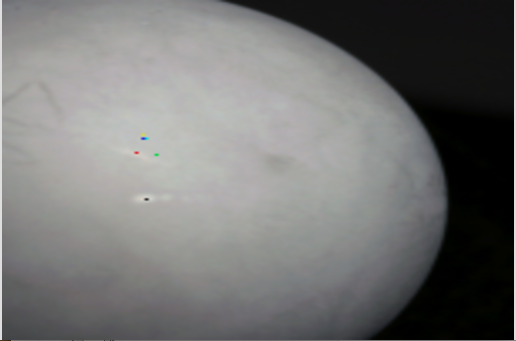
\includegraphics[scale=0.6]{ejemplo.png}
   \caption{Vecindades con ...}
   \label{Fig. 1}
\end{figure}

\indent La imágen se observan esos factores de los que hablamos en el desarrollo, entre aquellos, las manchas de distinto color y la aureola de luz. Pór ejemplo se ve el de vecindad 0 (púnto negro) bién lejos de los demas, por lo claro de la mancha blanca. Las vecindades de 2 y 4 (rojo y verde) también fueron corrompidos por el ruido, aunque llegaron un poco mas cerca. Luego a partir de los 6, 8 y 10 (azúl, amaríllo y cian) se podria creer que llega a un lugar en donde por más que agrandes el número de cantidad de vecindades no modificaria la posición, también viéndolo a simple vista se puede corroborar que es de dónde uno diria que proviene la luz.
\\
Prosiguiendo con las misma idea y utilizando las direcciones de luz obtenidas con vecindad 0 y vecindad 6,la cual consideramos la optima, obtuvimos distintos campos normales para la imágen del buda, observables a continuación:


\begin{figure}[h]
   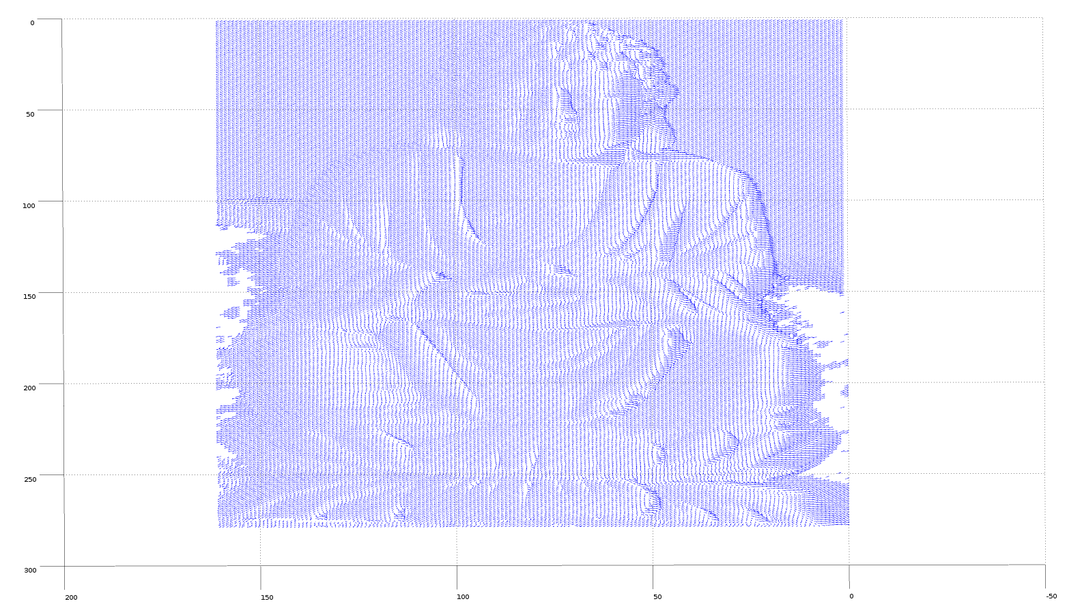
\includegraphics[scale=0.4]{buda_vecindad_0.png}
   \label{Fig. 2}
   \caption{Buda con vecindad 0}
\end{figure}

\begin{figure}[h]
   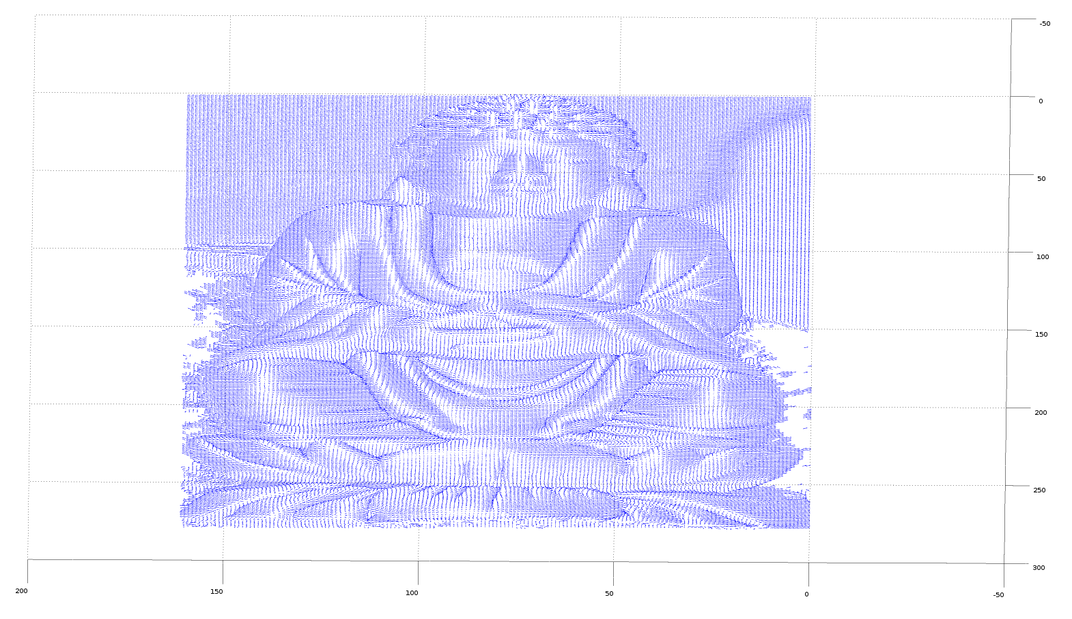
\includegraphics[scale=0.4]{buda_vecindades_6.png}
   \label{Fig. 3}
   \caption{Buda con vecindad 6}
\end{figure}



Concluimos con que modificar la cantidad de vecindades repercute fuertemente en la realización del resto del modelo, ya que con una mala dirección de la luz se perdera el efecto 3D, o mas bien parecera como que se obtuvo el efecto solo de uno de los lados (de derecha a izquierda). \par



\section{Número de condición}

La mejor forma de ver la diferencia entre dos matrices con distintos números de condición fue tomar la matrices con menor y con mayor número de condición asociados. De esta manera obtuvimos una matriz con un número de 15.0503 y otro con 407.581, una gran diferencia de tamaños. Luego para poder observar visualmente la dicerencia se le calculo el campo normal a cada uno, el resultado es el siguiente:



\begin{figure}[h]
   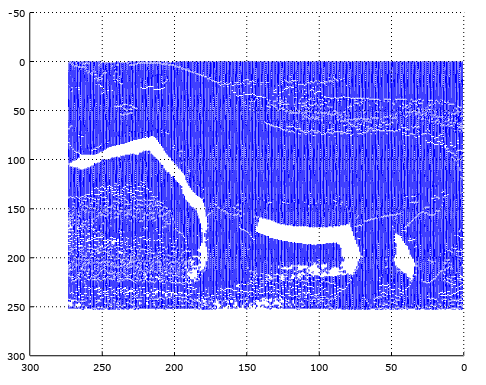
\includegraphics[scale=0.5]{caballoMax.png}
   \label{Fig. 4}
   \caption{Caballo con Número de condición de 407.581}
\end{figure}

\begin{figure}[h]
   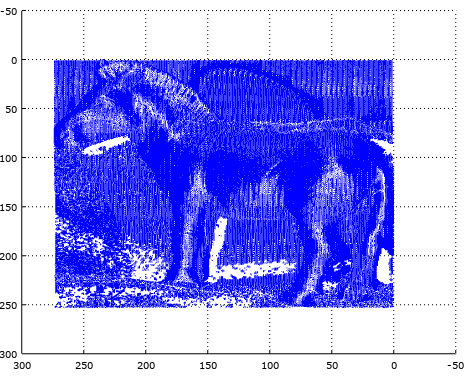
\includegraphics[scale=0.5]{caballoMin.png}
   \label{Fig. 5}
   \caption{Caballo con Número de condición de 15.0503}
\end{figure}


\section{Complejidades algoritmicas}

\indent Nuestra primer idea para tratar de comprobar nuestra hipótesis de que la factorización LU es mas rápida que la eliminación de gauss fue tomar distintos tamaños de matrices y triangularlos una vez con cada algoritmo para ver que método era mas rápido. Este experimento no pone a prueba nuestra hipótesis porque lo que intentábamos comprobar es que la factorización LU es mas rápida que la eliminación de gauss para resolver un sistema lineal despues de la primera vez que se resuelve el sistema. Si resolvíamos una sola vez cada tamaño de matriz, ambos algoritmos tardarían lo mismo. Por lo tanto, decidimos hacer un experimento donde mantuvimos constante el tamaño del sistema lineal a resolver y lo que variamos en cada instancia de testeo fueron las cantidades de términos independientes que debia resolver. Agregamos al mismo experimento la factorización de Cholesky.

\begin{figure}[h]
   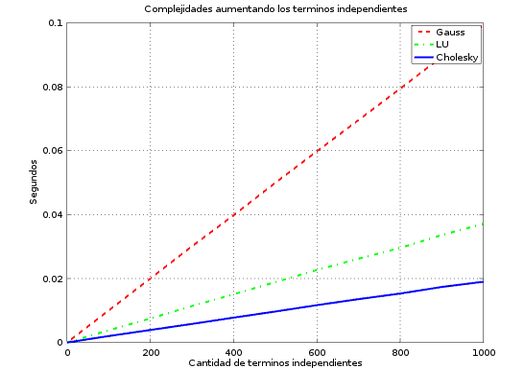
\includegraphics[scale=0.5]{ComplejidadesMalas.png}
   \label{Fig. 6}
   \caption{Resultado obtenido al aumentar la cantidad de terminos independientes}
\end{figure}

\indent Nuestra hipótesis, y a partir de lo que nos comentaron en las clases era que los algoritmos de eliminación gaussiana, factorización LU y Cholesky iban a tener un orden de complejidad cúbico y cuadrado, respectivamente, lo que al ver los resultados de las experimentaciones nos dice lo contrario. Las complejidades nos resultaron lineales.
Luego de consultarlo con la catedra, pudimos comprender que las complejidades no se iban a ver reflejadas en este experimento, ya que el tamaño de la matriz se mantenia igual. Por lo tanto debimos realizar un nuevo experimento en donde dejamos fijos en 100 terminos independientes a resolver y lo que se variaba en cada corrida era el tamaño de las matrices.


\begin{figure}[h]
   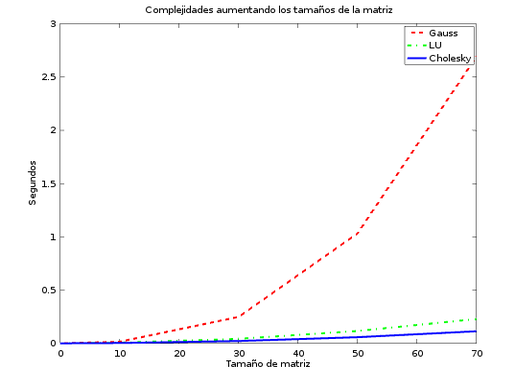
\includegraphics[scale=0.5]{complejidadesCorrecto.png}
   \label{Fig. 7}
   \caption{Resultado obtenido al aumentar la cantidad de terminos independientes}
\end{figure}

%\section{Discusi\'on}

%\subsection{Calibraci\'on}

\indent La imágen en la cual vimos la mayor diferencia es en Mate.6, d\'onde se observan esos factores de los que hablamos en el desarrollo, entre aquellos, las manchas de distinto color y la aureola de luz. P\'or ejemplo se ve el de vecindad 0 (p\'unto negro) bi\'en lejos de los demas, por lo claro de la mancha blanca. Las vecindades de 2 y 4 (rojo y verde) tambi\'en fueron corrompidos por el ruido, aunque llegaron un poco mas cerca. Luego a partir de los 6, 8 y 10 (az\'ul, amar\'illo y cian) se podria creer que llega a un lugar en donde por m\'as que agrandes el n\'umero de cantidad de vecindades no modificaria la posici\'on, tambi\'en vi\'endolo a simple vista se puede corroborar que es de d\'onde uno diria que proviene la luz.
Luego en el pr\'oximo experimento se observa que al modificar la cantidad de vecindades repercute fuertemente en la realizacion del resto del modelo, ya que con una mala direcci\'on de la luz se perdera el efecto 3D. \par

\subsection{Complejidades}

\indent Nuestra hipotesís, y a partir de lo que nos comentaron en las clases era que los algoritmos de eliminación gaussiana, factorización LU y Cholesky iban a tener un orden de complejidad cúbico y cuadrado, respectivamente, lo que al ver los resultados de las experimentaciones nos dice lo contrario. Las complejidades nos resultaron lineales, lo cual al pensarlo un momento se nos ocurrio que lo que puede estar pasando es debido a que la pendiente crece poco, a lo que deber\'iamos utilizar una cantidad may\'or de t\'erminos independientes. Esto \'ultimo no lo pudimos comprobar por falta de tiempo.  \par


\subsection{N\'umero de condici\'on}


\indent Nuestra hipótesis de que el n\'umero de condici\'on afecta directamente la estimaci\'on de las normales se puede ver confirmada claramente en las im\'agen del caballo. El campo de normales del caballo  en las figuras 1  esta estimado con la elección de direcciones de iluminaci\'on que causan que la matriz de la ecuaci\'on 5 tenga el m\'aximo n\'umero de condici\'on en comparaci\'on a todas las otras posibles combinaciones de direcciones. En contraste la figura 2 utiliza la conbinaci\'on de direcciones de iluminaci\'on que generan la matriz con el mejor n\'umero de condici\'on. Esto se da porque un n\'umero de condici\'on alto implica que las direcciones de iluminación est\'an apuntando desde una posici\'on muy similar lo cual es equivalente a tener una sola direcci\'on para generar las normales y tambi\'en las profundidades. \par

\subsection{RGB}

\indent La visi\'on humana tiende a diferenciar m\'as escalas de verde lo cual hace que al hacer un promedio ponderado para el color verde se obtengan mejores resultados. Esto lo tomamos en cuenta al momento de promediar los colores de los pixeles para buscar la direcci\'on proveniente de la luz. Al no poder encontrar una gran diferencia, decidimos utilizarlo.
(lo cuales no pudimos verlos en las imagenes que probamos)

//¿Como afectan la estimacion de las profundidades el calculo de las normales?


//¿Que metodos de solucion de los sistemas lineales arrojan mejores calculos de profundidades?

Aca escribimos las conclusiones.
¿Como afecta la calibracion del sistema en el resto de las etapas?
La calibracion es la parte inicial y fundamental para la resolucion de la reconstruccion 3D, ya que en ella obtenemos las direcciones de fuente de luz que afectara directamente al resultado, independientemente de que tan bueno sea el algoritmo para resolver sistemas lineales o estimar valores.

¿Como impacta la eleccion de las 3 direcciones de iluminacion para el calculo de las normales?
la eleccion de las direcciones de iluminacion afectara directamente a las normales ya que se aproximan apartir de ellas y si la matriz esta mal condicionada dara resultados no muy buenos.

\section{Conclusiones}



Las conclusiones finales de este trabajo desde principio a fin son las siguientes:
\begin{itemize}
\item Al momento de la calibración de la im\'agen es fundamental tomar bien las medidas, ya que si se arrastra este error, a medida que se le aplican los m\'etodos se potencia.
\item Se debe seleccionar de buena manera las direcciones de luz para eliminar las mayores posibilidades de tener alg\'un error de redondeo al medir las normales.
\item Al momento de calcular las profundidades se debe ser inteligente y poder rebuscarse para no consumir tanta memoria, ya que se trabajan con matrices demasiado grandes para tenerlas en memoria. En este paso es fundamental trabajar con matrices esparzas ya que poseen una gran cantidad de ceros.
\end{itemize}

%\section{Ap\'endices}

%Aca escribimos el apendices.

\section{Referencias}

1-Numerical Analysis - 9th Edition - (Burden and Faires)

\end{document}
